%%%%%%%%%%%%%%%%%%%%%%%%%%%%%%%%%%%%%%%%%
% Structured General Purpose Assignment
% LaTeX Template
%
% This template has been downloaded from:
% http://www.latextemplates.com
%
% Original author:
% Ted Pavlic (http://www.tedpavlic.com)
%
% Note:
% The \lipsum[#] commands throughout this template generate dummy text
% to fill the template out. These commands should all be removed when 
% writing assignment content.
%
%%%%%%%%%%%%%%%%%%%%%%%%%%%%%%%%%%%%%%%%%

\documentclass{article}

\usepackage{fancyhdr} % Required for custom headers
\usepackage{lastpage} % Required to determine the last page for the footer
\usepackage{extramarks} % Required for headers and footers
\usepackage{graphicx} % Required to insert images
\usepackage[utf8]{inputenc}

% Margins
\topmargin=-0.45in
\evensidemargin=0in
\oddsidemargin=0in
\textwidth=6.5in
\textheight=9.0in
\headsep=0.25in 

\linespread{1.1} % Line spacing



\setlength\parindent{0pt} % Removes all indentation from paragraphs

%----------------------------------------------------------------------------------------
%	DOCUMENT STRUCTURE COMMANDS
%	Skip this unless you know what you're doing
%----------------------------------------------------------------------------------------

% Header and footer for when a page split occurs within a problem environment
\newcommand{\enterProblemHeader}[1]{
\nobreak\extramarks{#1}{#1 continued on next page\ldots}\nobreak
\nobreak\extramarks{#1 (continued)}{#1 continued on next page\ldots}\nobreak
}

% Header and footer for when a page split occurs between problem environments
\newcommand{\exitProblemHeader}[1]{
\nobreak\extramarks{#1 (continued)}{#1 continued on next page\ldots}\nobreak
\nobreak\extramarks{#1}{}\nobreak
}

\setcounter{secnumdepth}{0} % Removes default section numbers
\newcounter{homeworkProblemCounter} % Creates a counter to keep track of the number of problems

%----------------------------------------------------------------------------------------
%	NAME AND CLASS SECTION
%----------------------------------------------------------------------------------------

\newcommand{\lessonNumber}[1]{Lezione\ \##1} % Assignment title
\newcommand{\lessonDate}[4]{#1,\ #2\ #3\ #4} % Due date
\newcommand{\lessonCourse}[1]{#1} % Course/class
\newcommand{\lessonTime}[1]{#1} % Class/lecture time
\newcommand{\lessonTeacher}[1]{#1} % Teacher/lecturer
\newcommand{\lessonAuthor}[1]{#1} % Your name
\begin{document}
\section{Gestione di Progetto(4)}

Fondamenti della \textbf{Gestione di progetto:}
\begin{enumerate}
	\item Introdurre processi nel progetto (introdurre disciplina);
	\item Stimare i costi e le risorse necessarie (avere una pianificazione preventiva) infatti un progetto diventa fattibile se la stima e accettabile;
	\item Pianificazione e assegnazione delle attività;
	\item Controllare le attività e verificare i risultati (avere chiaro e presente lo stato di avanzamento), non devo fare un pull \textit{chiedere} deve essere già tutto pronto. L'uso di \textbf{Milestone} aiuta a capire la differenza tra attesa e realtà.
\end{enumerate}

Per molto tempo si è pensato che i sw fossero repliche uniche ("\textit{one off}"); grave errore creare cose che siano irripetibili, la nostra attività prevalente sarà la \textit{manutenzione}.

Vediamo alcuni \textbf{Fattori di rischio} per la gestione di progetto:

\begin{itemize}

	\item \textbf{Variabilità nel personale:} nella disponibilità e nella composizione del team. Le persone possono "\textit{sparire}", a quel punto bisogna trovare un rimpiazzo;
	
	\item \textbf{Tecnologia:} due tecniche: chi usa solo tecnologie consolidate, e chi usa tecnologia innovativa (per motivi di competizione) ma fortemente instabile. Questa variabilità è un grande rischio.
	
	\item \textbf{Mercato:} competizione sul mercato.
	\item \textbf{Requisiti:} possono cambiare;
	\item \textbf{Specifiche:} ritardo nella presentazione;

\end{itemize}
Gli ultimi due sono facilmente evitabili con un'adeguata gestione dei rischi che va pianificata sia all'inizio che in corso d'opera in quanto possono variare nel tempo (analisi di probabilità che emergano). Ecco come pianificare una buona gestione dei rischi:

\begin{enumerate}

	\item \textbf{Identificazione:} capire quali sono nelle varie categorie specificate sopra;
	
	\item \textbf{Analisi:} probabilità di occorrenza;
	
	\item \textbf{Pianificazione:} come evitare i rischi;
	
	\item \textbf{Controllo:} attenzione continua tramite rilevazione di indicatori.

\end{enumerate}

Il team necessita di \textbf{ruoli}, che identificano capacità e compiti. Un ruolo è la \textit{funzione aziendale} assegnata al progetto. Vediamo alcuni ruoli:

\begin{itemize}

	\item \textbf{Qualità:} ciò che ci consente di puntare al miglioramento continuo di efficienza ed efficacia. Qualità di prodotto è diverso da qualità di processo. E' più importante la qualità di processo;
	
	\item \textbf{Sviluppo:} insieme delle competenze per la parte di attività tecnica e realizzativa del prodotto;
	
	\item \textbf{Direzione:} fa sì che l'organizzazione possa stare in piedi;
	
	\item \textbf{Amministrazione:} ("\textit{service manager}") erogano/gestiscono l'infrastruttura che aiuta a fare il proprio lavoro (es. manutenzione e sicurezza). Se esiste una buona infrastruttura si lavora meglio.

\end{itemize}

Competenze allo richieste:

\begin{itemize}

	\item \textbf{Analista:} colui che serve per fare analisi dei requisiti; aiuta l'avanzamento di maturità dei requisiti; bisogna avere competenze su più fronti, sapere ascoltare gli \textit{stakeholder}, scrivere requisiti \textit{bounded} e \textit{coherent}, ragionevoli, utili, realizzabili e verificabili. Hanno un gran peso sul successo del progetto; l'analista pensa al problema, non alla soluzione;
	
	\item \textbf{Progettista:} pensa alla soluzione. Deve avere competenze tecnologiche e tecniche. Ricevuto il problema elabora la migliore soluzione possibile nel rispetto dei vincoli finanziari e temporali. Deve sapere di architettura, mettere insieme le parti della soluzione (divide et impera), rendere il problema piccolo affinché sia dominabile. Un solo progettista in un team;
	
	\item \textbf{Programmatori:} hanno responsabilità e visione circoscritte, il passaggio di consegna tra progettista e programmatore deve essere chiaro. Partecipano anche alla manutenzione. Ho tanti programmatori quanti posso averne;
	
	\item \textbf{Verificatori:} la validazione si fa sul prodotto finito. Impiega almeno 1/3 del tempo. Partecipano a tutto il ciclo di vita del progetto. Include anche la verifica del codice: 1) impone al programmatore stesso di verificare il suo codice, 2) lo fa verificare ad una terza persona indipendente;
	
	\item \textbf{Responsabile:} ce ne sarà 1. Rappresenta il progetto presso il fornitore e presso il committente. E' quello che fa da intermediario, che dice "\textit{come siamo messi}"; pianifica, gestisce risorse e rischi, coordina. Responsabilità su relazioni esterne. Deve sapere ciò di cui parla. Diventa responsabile dopo avere acquisito esperienza su altri ruoli;
	
	\item \textbf{Amministratore:} ruolo molto utile, prepara l'ambiente di lavoro, strumenti di collaborazione e controllo di avanzamento. Gestione della documentazione di progetto. Risoluzione di problemi legati alla gestione di processi. Assegnazione di \textit{tickets}, un incarico con scadenza assegnato ed accettato.
\end{itemize}

\textbf{Gestione qualità:} la possiamo guardare da due punti di vista: qualità sul prodotto e qualità di processo (su ciò che si fa). E' una competenza strategica, una funzione aziendale e non un ruolo di progetto. Dobbiamo lavorare prima per fare meno manutenzione poi.

\textbf{Pianificazione di progetto:} per prima cosa devo definire le attività per pianificarne lo svolgimento e controllarne l'attuazione, per stimare e controllare scadenze e costi.
\\
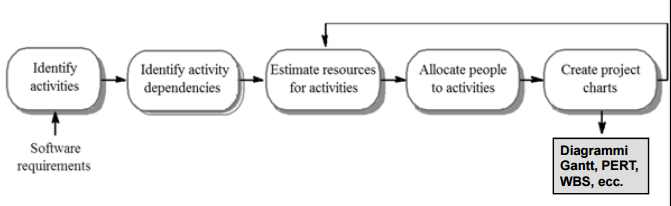
\includegraphics[width=0.75\columnwidth]{img8}

Si pianificano le attività, i flussi di attività e i flussi di azione. Le attività hanno un flusso, si dipanano su un asse temporale. Capite le attività devo assegnare ad esse dei ruoli (non come persone).Devo quantificare lao svolgere un'attività, data, tempo, persone, denaro. Le ore vanno intese come ore di calendario: tempo/persona, quanto tempo uso tali persone sapendo che ciascuna percepisce un costo orario preciso. In base a questo posso capire quanto mi costerà un progetto. Vediamo alcuni strumenti che aiutano la gestione:
\begin{itemize}
	\item \textbf{Diagrammi di Gantt:} sull'asse orizzontale c'è il tempo segmentato per unità di lavoro (es. 1gg, una settimana, un mese..). Una buona scelta è utilizzare come unità di misura un giorno (8 ore lavorative), ho anche un calendario (es. sabato e domenica non si lavora). Sull'asse orizzontale ci sono tutte le attività che devo svolgere e archi che rappresentano le transizioni tra una e l'altra. Le dipendenze logiche tra attività: quelle che non hanno dipendenze partono subito, la seconda è la durata minima di tempo/persone che posso usare per una determinata attività. Work allocation, in questa fase non sto allocando persone ma ruoli. Questo grafico permette di cofrontare le stime con i progressi;
	\item \textbf{Diagramma di PERT:} \fbox{\textbf{Def:} Program Evaluation and Review Technique} descrive le dipendenze temporali tra le attività, serve a trovare le criticità ossia dove ho delle dipendenze temporali strette. Se misuro lo slack e mi accorgo che è 0 o negativo ho una criticità. Indica l'ordine delle attività e la loro durata e indica la prima data in cui posso iniziare un'attività che abbia tutti gli input necessari. Calcolando il cammino più lungo tra l'inizio e la fine del progetto posso calcolare l'attività che finisce prima. Questo diagramma legge il Gantt rispetto allo slack e calcola i cammini critici;
	\item \textbf{Work Breakdown Structure:} si frantumano le attività in sotto attività e vengono organizzate in modo gerarchico. Ogni componente deve essere univocamente identificabile. Un'attività decomposta permette di agevolare il parallelismo.  Allocazione delle risorse: assegnare attività a ruoli e poi ruoli a persone per far si che ogni persona sia impegnata per tutto il tempo disponibile. Diagramma di Gantt ribaltato sulle persone (al posto delle attività); l'intento è sapere che sto usando le persone in parallelo ed entro il limite dato.
\end{itemize}

Fattori di influenza che fanno aumentare il tempo/persona:
\begin{itemize}
	\item \textbf{Dimensione del progetto:} quante righe di codice mi servono, la dimensione si riesce a stimare macroscopicamente; sta tra due assi: quanto codice e quanto complesso;
	\item \textbf{Esperienza del dominio:} quanta è l'esperienza (normativa, tecnologica, aspettative degli utenti) di chi svolge il progetto nei confronti del dominio a cui siamo davanti;
	\item \textbf{Tecnologie adottate:} influenza molto forte, è una scelta strategica di amministrazione, si cerca stabilità e maturità;
	\item \textbf{Ambiente di sviluppo:} procedure e tecniche con le quali collaboriamo, dobbiamo collocale a basso costo temporale;
	\item \textbf{Qualità dei processi richiesta}
\end{itemize}

Uno dei problemi più difficili da risolvere sono le \textbf{Problematiche di stima}:
\begin{itemize}
	\item \textbf{Legge di Parkinson:} il lavoro si espande fino a riempire il tempo disponibile;
	\item \textbf{Legge della domanda:} l'utilità determina il prezzo
\end{itemize}



\end{document}
